\documentclass[tikz,border=0pt]{standalone}
\usepackage{amsmath, amssymb}
\usetikzlibrary{matrix, positioning, fit, backgrounds, calc}
\usepackage{helvet}
\usepackage{avant}
\renewcommand*\familydefault{\sfdefault}
\usepackage{textcomp}

\usepackage{fontspec}
\setmainfont{TeX Gyre Termes}
\setsansfont[
Path = fonts/,
UprightFont = *Medium.ttf,
BoldFont    = *Bold.ttf,
AutoFakeSlant = 0.2
]{GmarketSansTTF}
\begin{document}
	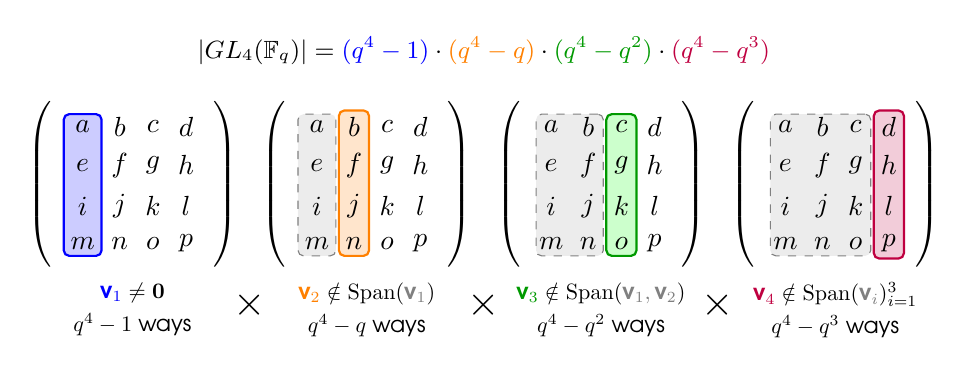
\begin{tikzpicture}[
		font=\sffamily,
		% Style for the matrices
		mtx/.style={
			matrix of math nodes,
			left delimiter=(, right delimiter=),
			nodes={minimum width=1em, inner sep=2pt, anchor=center},
			column sep=2pt, row sep=2pt,
			ampersand replacement=\&
		},
		% Highlighting styles for active columns
		hl-v1/.style={fill=blue!20, draw=blue, thick, rounded corners=2pt, inner sep=.25pt},
		hl-v2/.style={fill=orange!20, draw=orange, thick, rounded corners=2pt, inner sep=.25pt},
		hl-v3/.style={fill=green!20, draw=green!60!black, thick, rounded corners=2pt, inner sep=.25pt},
		hl-v4/.style={fill=purple!20, draw=purple, thick, rounded corners=2pt, inner sep=.25pt},
		% Style for the accumulating "Span Box"
		hl-span/.style={fill=gray!15, draw=gray, dashed, rounded corners=2pt, inner sep=.25pt},
		% Title & Text
		mainTitle/.style={font=\sffamily\bfseries\LARGE, color=darkgray, align=center},
		term label/.style={font=\bfseries\small, align=center}
		]

	% ==============================================================================
	% ROW 3: m = 4 (Generalizing)
	% ==============================================================================
	\begin{scope}[shift={(-4.5, -5.5)}, scale=0.85]
		\node[term label] at (5.25, 2.0) {$|GL_4(\mathbb F_q)| = \textcolor{blue}{(q^4-1)} \cdot \textcolor{orange}{(q^4-q)} \cdot \textcolor{green!60!black}{(q^4-q^2)} \cdot \textcolor{purple}{(q^4-q^3)}$};
		
		% Col 1
		\matrix[mtx] (M4_1) at (0, 0) {
				a \& b \& c \& d \\
				e \& f \& g \& h \\
				i \& j \& k \& l \\
				m \& n \& o \& p \\
			}; 
		\begin{scope}[on background layer] \node[hl-v1, fit=(M4_1-1-1)(M4_1-4-1)] {}; \end{scope}
		\node[below=0.1cm of M4_1, align=center, scale=0.8] {
				$\textcolor{blue}{\textbf{v}_1} \neq \mathbf{0}$ \\[1mm]
				\textbf{$q^4 - 1$} ways
			};
		
		% Col 2
		\matrix[mtx] (M4_2) at (3.5, 0) {
				a \& b \& c \& d \\
				e \& f \& g \& h \\
				i \& j \& k \& l \\
				m \& n \& o \& p \\
			};
		\begin{scope}[on background layer]
				\node[hl-span, fit=(M4_2-1-1)(M4_2-4-1)] {};
				\node[hl-v2, fit=(M4_2-1-2)(M4_2-4-2)] {};
			\end{scope}
		\node[below=0.1cm of M4_2, align=center, scale=0.8] {
				$\textcolor{orange}{\textbf{v}_2} \notin \mathrm{Span}(\textcolor{gray}{\textbf{v}_1})$ \\[1mm]
				\textbf{$q^4 - q$} ways
			};
		
		% Col 3
		\matrix[mtx] (M4_3) at (7.0, 0) {
				a \& b \& c \& d \\
				e \& f \& g \& h \\
				i \& j \& k \& l \\
				m \& n \& o \& p \\
			};
		\begin{scope}[on background layer]
				\node[hl-span, fit=(M4_3-1-1)(M4_3-4-2)] {};
				\node[hl-v3, fit=(M4_3-1-3)(M4_3-4-3)] {};
			\end{scope}
		\node[below=0.1cm of M4_3, align=center, scale=0.8] {
				$\textcolor{green!60!black}{\textbf{v}_3} \notin \mathrm{Span}(\textcolor{gray}{\textbf{v}_1, \textbf{v}_2})$ \\[1mm]
				\textbf{$q^4 - q^2$} ways
			};
		
		% Col 4
		\matrix[mtx] (M4_4) at (10.5, 0) {
				a \& b \& c \& d \\
				e \& f \& g \& h \\
				i \& j \& k \& l \\
				m \& n \& o \& p \\
			};
		\begin{scope}[on background layer]
				\node[hl-span, fit=(M4_4-1-1)(M4_4-4-3)] {};
				\node[hl-v4, fit=(M4_4-1-4)(M4_4-4-4)] {};
			\end{scope}
		\node[below=0.1cm of M4_4, align=center, scale=0.8] {
				$\textcolor{purple}{\textbf{v}_4} \notin \mathrm{Span}(\textcolor{gray}{\textbf{v}_i})_{i=1}^3$ \\[1mm]
				\textbf{$q^4 - q^3$} ways
			};
		
		% Draw multiplication signs after nodes exist
		\node[scale=1.5] at ($(M4_1)!0.5!(M4_2)+(0,-1.8)$) {$\times$};
		\node[scale=1.5] at ($(M4_2)!0.5!(M4_3)+(0,-1.8)$) {$\times$};
		\node[scale=1.5] at ($(M4_3)!0.5!(M4_4)+(0,-1.8)$) {$\times$};
	\end{scope}
	\end{tikzpicture}
\end{document}